

%% AAPT Physics Bowl Exams Questions
%%----------------------------------------


%% This section has XX problems


%% PhysicsBowl 2015
%%----------------------------------------
\element{aapt}{ %% Bowl-D5
\begin{question}{bowl-2015-q37}
    Which one of the following choices represents the base SI units of inductance?
    \begin{multicols}{3}
    \begin{choices}
      \correctchoice{$\dfrac{\si{\kilo\gram\meter\squared}}{\si{\ampere\squared\second\squared}}$}
        \wrongchoice{$\dfrac{\si{\kilo\gram\meter\squared}}{\si{\ampere\second}}$}
        \wrongchoice{$\dfrac{\si{\kilo\gram\meter}}{\si{\ampere\squared\second\squared}}$}
        \wrongchoice{$\dfrac{\si{\kilo\gram\meter\squared}}{\si{\ampere\squared\second\cubed}}$}
        \wrongchoice{$\dfrac{\si{\kilo\gram\meter}}{\si{\ampere\squared\second\cubed}}$}
    \end{choices}
    \end{multicols}
\end{question}
}

\element{aapt}{ %% Bowl-D5
\begin{question}{bowl-2015-q50}
    A magnetic field directed into the plane of the page is decreasing in time.
    A constant emf $\xi$ is produced for the square loop enclosing the field in the figure.
    \begin{center}
    \ctikzset{bipoles/length=0.75cm}
    \begin{circuitikz}
        %% circuit
        \draw (0,0) to [voltmeter] (4,4) to (4,0);
        \draw (0,0) to (0,4) to [R,l=$R$] (2,4) to [R,l=$R$] (4,4) to (4,0) to [R,l=$R$] (0,0);
        %% B field into page
        \foreach \x in {0.5,1.0,...,3.5}
            \foreach \y in {0.5,1.0,...,3.5}
                \foreach \i in {45,135,225,315} {
                    \pgfmathifthenelse{\x==\y}{}{"\noexpand\draw[thick] (\x,\y) -- ++(\i:0.1);"}\pgfmathresult
                }
    \end{circuitikz}
    \end{center}
    The square loop has three identical light bulbs of resistance $R$
        in it and an ideal voltmeter connected to the corners through the center of the loop.
    What is the magnitude of the voltmeter's reading?
    \begin{multicols}{3}
    \begin{choices}
        \wrongchoice{$0\xi$}
        \wrongchoice{$\dfrac{1}{2}\xi$}
        \wrongchoice{$\dfrac{1}{3}\xi$}
      \correctchoice{$\dfrac{1}{6}\xi$}
        \wrongchoice{$\dfrac{2}{3}\xi$}
    \end{choices}
    \end{multicols}
\end{question}
}


%% PhysicsBowl 2014
%%----------------------------------------
\element{aapt}{ %% Bowl-D5
\begin{question}{bowl-2014-q34}
    Two circular loops of resistive wire are placed next to each other as in the figure.
    \begin{center}
    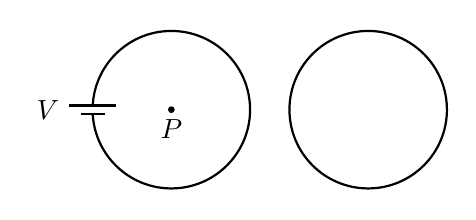
\begin{tikzpicture}
        %% Battery
        \node[anchor=east] at (180:1.30cm) {$V$};
        %% Left Circle
        \draw[thick] (177:1cm) -- ++ (0:0.30cm);
        \draw[thick] (177:1cm) -- ++ (180:0.30cm);
        \draw[thick] (-177:1cm) -- ++ (0:0.15cm);
        \draw[thick] (-177:1cm) -- ++ (180:0.15cm);
        \draw[thick] (-177:1cm) arc (-177:177:1cm);
        %% Right Circle
        \draw[thick] (2.5,0) circle (1cm);
        \draw[fill] (0,0) circle (1pt) node[anchor=north] {$P$};
    \end{tikzpicture}
    \end{center}
    The circular loop on the left is connected to a constant voltage source $V$.
    The resistance of this loop is increasing linearly with time.
    As the resistance is changing,
        what is the direction of the magnetic field at point $P$ (the center of the left-hand loop) and what is the orientation of the conventional current in the right-hand loop (as viewed in the figure from above)?
    \begin{center}
    \begin{tabu}{cX[5c]X[4c]}
        \toprule
        \makebox[1.5em][c]{\textnumero}
            & Magnetic Field Direction
            & Current Orientation \\
        \bottomrule
    \end{tabu}
    \end{center}
    \begin{choices}
      \correctchoice{\begin{tabu}{X[5c]X[4c]} Into the plane of the page & Counterclockwise \\ \end{tabu}}
        \wrongchoice{\begin{tabu}{X[5c]X[4c]} Into the plane of the page & Clockwise \\ \end{tabu}}
        \wrongchoice{\begin{tabu}{X[5c]X[4c]} Out of the plane of the page & Counterclockwise \\ \end{tabu}}
        \wrongchoice{\begin{tabu}{X[5c]X[4c]} Out of the plane of the page & Counterclockwise \\ \end{tabu}}
        \wrongchoice{\begin{tabu}{X[5c]X[4c]} There is no field & There is no current \\ \end{tabu}}
    \end{choices}
\end{question}
}


%% PhysicsBowl 2013
%%----------------------------------------
\element{aapt}{ %% Bowl-D5
\begin{question}{bowl-2013-q35}
    For the figure shown,
        the variable resistance of the inner circuit,
        $R_{\text{inner}}$, is increasing at a constant rate.
    \begin{center}
    \ctikzset{bipoles/length=0.75cm}
    \begin{circuitikz}[scale=1.00]
        %% outer circuit
        \draw (-3,-2) to (-3,2) to [R,l=$R_{\text{outer}}$] (3,2) to (3,-2) to (-3,-2);
        \fill (-3,2) circle (2pt) node[anchor=south] {$X$};
        \fill (+3,2) circle (2pt) node[anchor=south] {$Y$};
        %% inbetween
        \fill (-2.5,-1.5) circle (2pt) node[anchor=south] {$P$};
        %% inner circuit
        \draw (-2,-1) to (-2,1) to (2,1) to (2,-1) to [battery,l=$V$] (0,-1) to [vR,l=$R_{\text{inner}}$] (-2,-1);
    \end{circuitikz}
    \end{center}
    While this is occurring,
    in which direction is the magnetic field associated with the inner circuit at the point $P$ in the plane of the circuit and in which direction is the flow of electrons through the resistor labeled $R_{\text{outer}}$?
    \begin{center}
    \begin{tabu}{cX[c]X[c]}
        \toprule
        \makebox[1.5em][c]{\textnumero}
        & Magnetic Field at $P$ & Electron flow through $R_{\text{outer}}$ \\
        \bottomrule
    \end{tabu}
    \end{center}
    \begin{choices}
        \wrongchoice{\begin{tabu}{X[c]X[c]} There is no field & There is no flow \\ \end{tabu}}
        \wrongchoice{\begin{tabu}{X[c]X[c]} Into the page & From $Y$ to $X$ \\ \end{tabu}}
      \correctchoice{\begin{tabu}{X[c]X[c]} Into the page & From $X$ to $Y$ \\ \end{tabu}}
        \wrongchoice{\begin{tabu}{X[c]X[c]} Out of the page & From $Y$ to $X$ \\ \end{tabu}}
        \wrongchoice{\begin{tabu}{X[c]X[c]} Out of the page & From $X$ to $Y$ \\ \end{tabu}}
    \end{choices}
\end{question}
}


%% PhysicsBowl 2012
%%----------------------------------------
\element{aapt}{ %% Bowl-D5
\begin{question}{bowl-2012-q38}
    A squared, conducting wire loop sits in a plane perpendicular to
        a spatially uniform magnetic field pointing into the plane
        of the page as shown.
    The magnetic field strength steadily increases with time.
    \begin{center}
    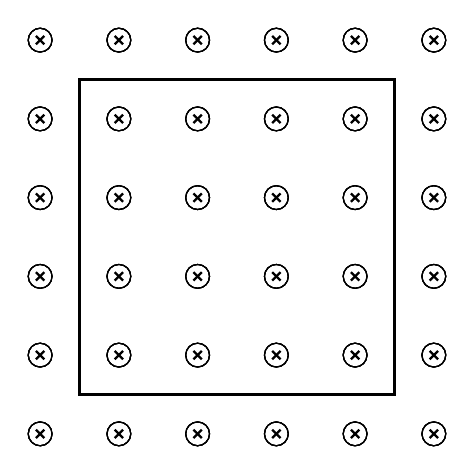
\begin{tikzpicture}
        %% B field into page
        \foreach \x in {-25,-15,...,25}
            \foreach \y in {-25,-15,...,25}
                \foreach \a in {45,135,225,315} {
                    \draw[thin] (\x mm,\y mm) circle (1ex);
                    \draw[thick] (\x mm,\y mm) -- ++(\a:0.5ex);
                }
        %% rectangular loop
        \draw[very thick] (-2,-2) rectangle (2,2);
    \end{tikzpicture}
    \end{center}
    Which one of the following effects best describes the result
        of this field increase?
    \begin{choices}
        \wrongchoice{The entire loop moves up the plane of the page.}
        \wrongchoice{The loop rotates with the top of the loop initially moving out of the plane of the page and the bottom edge moving into the plane of the page.}
        \wrongchoice{The loop rotates with the top of the loop initially moving into the plane of the page and the bottom edge moving out of the plane of the page.}
        \wrongchoice{The legs of the loop attempt to increase the area enclosed by the loop.}
      \correctchoice{The legs of the loop attempt to decrease the area enclosed by the loop.}
    \end{choices}
\end{question}
}

\element{aapt}{ %% Bowl-D5
\begin{question}{bowl-2012-q50}
    A spatially uniform electric field is constrained within the circular region of radius $R$ as shown.
    \begin{center}
    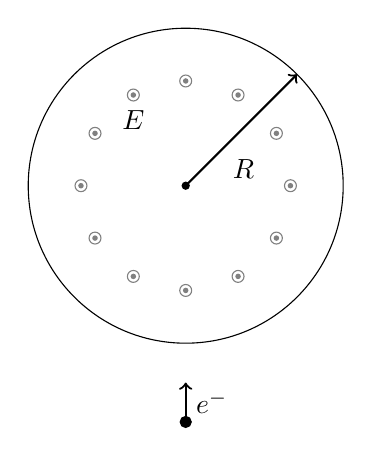
\begin{tikzpicture}
        %% E field
        \foreach \a in {0,30,...,330}
            \foreach \r in {1.33} {
                \draw[gray] (\a:\r) circle  (0.5ex);
                \fill[gray] (\a:\r) circle  (1pt);
            }
        \node[anchor=north,yshift=-0.5ex] at (120:1.33) {$E$};
        %% circle
        \draw (0,0) circle (2);
        \fill (0,0) circle (1.5pt);
        \draw[thick,->] (0,0) -- (45:2) node[pos=0.33,anchor=north west] {$R$};
        %% electron
        \draw[fill] (0,-3) circle (2pt);
        \draw[thick,->] (0,-3) -- ++(90:0.5) node[pos=0.5,anchor=west] {$e^{-}$};
    \end{tikzpicture}
    \end{center}
    The field is directed out of the plane of the page and its strength is decreasing uniformly with time.
    Which one of the following choices best represents the direction of the Lorentz force on the electron at the instant shown in the figure when the electron is moving up the plane of the page?
    Ignore gravity.
    \begin{choices}
        \wrongchoice{No Force}
      \correctchoice{Into to the plane of the page}
        \wrongchoice{Out of the plane of the page}
        \wrongchoice{To the right}
        \wrongchoice{To the left}
    \end{choices}
\end{question}
}


%% PhysicsBowl 2011
%%----------------------------------------
\element{aapt}{ %% Bowl-D5
\begin{question}{bowl-2011-q25}
    The product $\left(\SI{3}{\tesla}\times\SI{2}{\meter}\times\SI{4}{\meter\per\second}\right)$ is equivalent to which one of the following
    \begin{multicols}{3}
    \begin{choices}
        \wrongchoice{\SI{24}{\ampere}}
        \wrongchoice{\SI{24}{\coulomb}}
        \wrongchoice{\SI{24}{\watt}}
        \wrongchoice{\SI{24}{\ohm}}
      \correctchoice{\SI{24}{\volt}}
    \end{choices}
    \end{multicols}
\end{question}
}

\element{aapt}{ %% Bowl-D5
\begin{question}{bowl-2011-q41}
    For the figure show, the variable resistance of the outer circuit,
        $R_{\text{outer}}$, is decreasing at a constant rate.
    \begin{center}
    \ctikzset{bipoles/length=1.00cm}
    \begin{circuitikz}[scale=1.00]
        %% outer circuit
        \draw (-3,-2) to [vR,l=$R_{\text{outer}}$] (0,-2) to [battery,l=$V$] (3,-2) to (3,2) to (-3,2) to (-3,-2);
        %% inner circuit
        \draw (-2,-1) to (-2,1) to [R,l=$R_{\text{inner}}$] (2,1) to (2,-1) to (-2,-1);
        \fill (-2,1) circle (2pt) node[anchor=south] {$X$};
        \fill (+2,1) circle (2pt) node[anchor=south] {$Y$};
        %% inbetween
        \fill (0,+2.5) circle (2pt) node[anchor=south] {$P$};
    \end{circuitikz}
    \end{center}
    While this is occurring,
    in which direction is the magnetic field associated with the outer circuit at the point $P$ in the plane of the circuit and in which direction is the conventional current through the resistor $R_{\text{inner}}$ in the smaller interior circuit?  
    The two circuits lie on a flat table.
    \begin{center}
    \begin{tabu}{cX[c]X[c]}
        \toprule
        \makebox[1.5em][c]{\textnumero}
        & Magnetic Field at $P$ & Current through $R_{\text{inner}}$ \\
        \bottomrule
    \end{tabu}
    \end{center}
    \begin{choices}
      \correctchoice{\begin{tabu}{X[c]X[c]} Into the page & From $X$ to $Y$ \\ \end{tabu}}
        \wrongchoice{\begin{tabu}{X[c]X[c]} Into the page & From $Y$ to $X$ \\ \end{tabu}}
        \wrongchoice{\begin{tabu}{X[c]X[c]} Into the page & There is no current \ \end{tabu}}
        \wrongchoice{\begin{tabu}{X[c]X[c]} Out of the page & From $X$ to $Y$ \\ \end{tabu}}
        \wrongchoice{\begin{tabu}{X[c]X[c]} Out of the page & From $Y$ to $X$ \\ \end{tabu}}
    \end{choices}
\end{question}
}

\element{aapt}{ %% Bowl-D5
\begin{question}{bowl-2011-q48}
    An electromagnetic wave has a magnetic field given by the expression (in Cartesian coordinates)
    \begin{multline*}
        \vec{\mathbf{B}}\left(x,y,z,t\right) = \\
            \left(\num{6.0e-6}\right)\cos\left(\num{2.21e7}z-\num{6.63e15}t\right)\hat{x} \, .
    \end{multline*}
    At time $t=0$ and position $x=y=z=0$,
        what is the direction of the electric field associated with this wave?
    \begin{multicols}{3}
    \begin{choices}
        \wrongchoice{$+x$}
        \wrongchoice{$-x$}
        \wrongchoice{$+y$}
      \correctchoice{$-y$}
        \wrongchoice{$+z$}
    \end{choices}
    \end{multicols}
\end{question}
}


%% PhysicsBowl 2009
%%----------------------------------------
\element{aapt}{ %% Bowl-D5
\begin{question}{bowl-2009-q48}
    An electromagnetic wave has an electric field given
        by the expression (in Cartesian coordinates)
    \begin{equation*}
        \vec{E}(x,t) = \num{6.0} \cos\left(\num{1.14e7}x - \num{3.43e15}t \right) \hat{z}
    \end{equation*}
    %% start question
    What is the direction of the energy flow for the wave?
    \begin{multicols}{3}
    \begin{choices}
        \wrongchoice{$-x$}
      \correctchoice{$+x$}
        \wrongchoice{$-y$}
        \wrongchoice{$+y$}
        \wrongchoice{$+z$}
    \end{choices}
    \end{multicols}
\end{question}
}

\element{aapt}{ %% Bowl-D5
\begin{question}{bowl-2009-q49}
    An electromagnetic wave has an electric field given
        by the expression (in Cartesian coordinates)
    \begin{equation*}
        \vec{E}(x,t) = \num{6.0} \cos\left(\num{1.14e7}x - \num{3.43e15}t \right) \hat{z}
    \end{equation*}
    %% start question
    What is the direction of the magnetic field at time
        $t=\num{0}$ and position $x=\num{0}$?
    \begin{multicols}{3}
    \begin{choices}
        \wrongchoice{$-x$}
        \wrongchoice{$+x$}
      \correctchoice{$-y$}
        \wrongchoice{$+y$}
        \wrongchoice{$+z$}
    \end{choices}
    \end{multicols}
\end{question}
}


%% PhysicsBowl 2006
%%----------------------------------------
\element{aapt}{ %% Bowl-D5
\begin{question}{bowl-2006-q42}
    A solenoid is constructed with $N$ loops of wire tightly wrapped around an iron-filled center.
    Due to budget cuts, the current that ordinarily runs through this solenoid is cut in half.
    As a result, the inductance of the solenoid is:
    \begin{multicols}{2}
    \begin{choices}
      \correctchoice{unchanged.}
        \wrongchoice{quartered.}
        \wrongchoice{halved.}
        \wrongchoice{doubled.}
        \wrongchoice{quadrupled.}
    \end{choices}
    \end{multicols}
\end{question}
}


%% PhysicsBowl 2005
%%----------------------------------------
\element{aapt}{ %% Bowl-D5
\begin{question}{bowl-2005-q36}
    When one computes the square root of the ratio of the
        permeability of free space to the permittivity of free space,
        one obtains $\sqrt{\dfrac{\mu_0}{\epsilon_0}}=337$.
    What is the unit of this quantity?
    \begin{choices}
        \wrongchoice{farads (\si{\farad})}
        \wrongchoice{joules (\si{\joule})}
        \wrongchoice{volts (\si{\volt})}
        \wrongchoice{meters per second (\si{\meter\per\second})}
      \correctchoice{ohm (\si{\ohm})}
    \end{choices}
\end{question}
}


%% PhysicsBowl 2000
%%----------------------------------------
\element{aapt}{ %% Bowl-D5
\begin{questionmult}{bowl-2000-q10}
    When a wire moving through a magnetic field has a voltage induced between the wire's ends,
        that voltage is:
    \begin{choices}
      \correctchoice{directly proportional to the strength of the magnetic field.}
      \correctchoice{directly proportional to the velocity of the wire.}
        \wrongchoice{directly proportional to the diameter of the wire.}
    \end{choices}
\end{questionmult}
}


%% PhysicsBowl 1994
%%----------------------------------------
\element{aapt}{ %% Bowl-D5
\begin{question}{bowl-1994-q20}
     A magnet is dropped through a vertical copper pipe slightly larger than the magnet.
     Relative to the speed it would fall in air, the magnet in the pipe falls:
     \begin{choices}
         \wrongchoice{more slowly because it is attracted by the innate magnetic field of the pipe.}
       \correctchoice{more slowly because the currents induced in the pipe produce an opposing magnetic field.}
         \wrongchoice{at the same rate.}
         \wrongchoice{more quickly because it is attracted by the innate magnetic field of the pipe.}
         \wrongchoice{more quickly because the currents induced in the pipe produce a opposing magnetic field.}
    \end{choices}
\end{question}
}


\endinput


